\documentclass[color,hyper]{NRSMRev}

\NRSMsetup{
  stitle       = {Bare Demo of NRSMRev.cls for USNC-URSI National Radio Science Meeting},
  sauthor      = {Yuchen Jin, Yuchen Jin II},
  subject      = {URSI 2020},
  codeStyle    = {box},
  refNum       = {true}
}

\title{Bare Demo of NRSMRev.cls\\ for USNC-URSI National Radio Science Meeting}

% author names and affiliations
% use a multiple column layout for up to three different
% affiliations
\author{\IEEEauthorblockN{Authors Name/s associated with 1st Affiliation}
  \IEEEauthorblockA{line 1: dept. name (if applicable)\\
    line 2: name of organization, acronyms acceptable\\
    line 3: City, State/Province, Country\\
    line 4: e-mail address if desired\\}
  \and
  \IEEEauthorblockN{Authors Name/s associated with 2nd Affiliation}
  \IEEEauthorblockA{line 1: dept. name (if applicable)\\
    line 2: name of organization, acronyms acceptable\\
    line 3: City, State/Province, Country\\9444444444444787
    line 4: e-mail address if desired}}

%===========================================================
\begin{document}
	
\maketitle

\begin{abstract}
  The abstract goes here.
\end{abstract}

% Note that keywords are not normally used for peerreview papers.
\begin{IEEEkeywords}
  IEEE, IEEEtran, journal, \LaTeX, paper, template.
\end{IEEEkeywords}

\section{Show Homework}
sadfasf, sdfdsf, sdf.

Test citations:

\cite{Zeiler5539957}~\cite{Yang6175956}~\cite{Dong7115171}.

\subsection{Show Floats}

Test figures and example block which is shown in \autoref{ex1}.

\begin{example}[Figure Problem] \label{ex1}
  Test inner subgraphs, i.e. \autoref{fig:ex1:resD:a} and \autoref{fig:ex1:resD:b}. Also test \ref{fig:ex1:resD:b} and \eqref{fml:th1:partialW}:
  
  \begin{figure}[H] \label{fig:ex1:resD}
		\centering
		\begin{minipage}[b]{0.48\columnwidth}
			\centering
			\subfigure[$D=1$]{ \label{fig:ex1:resD:a}
				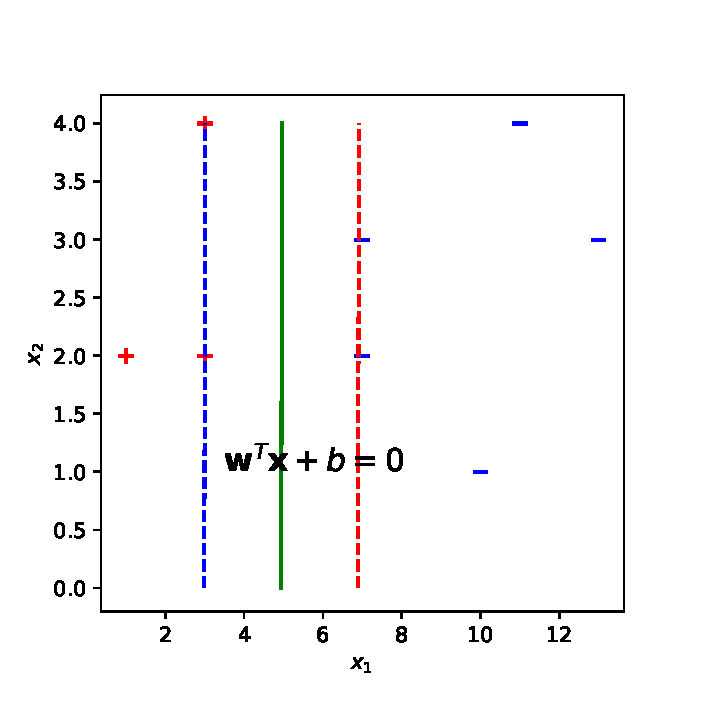
\includegraphics[width = 0.7\columnwidth]{pic-ex}
			}
		\end{minipage}
		\begin{minipage}[b]{0.48\columnwidth}
			\centering
			\subfigure[$D=0.5$]{ \label{fig:ex1:resD:b}
				Here could be graphs.
			}
		\end{minipage}
		\DeclareGraphicsExtensions.
		\caption{Test graphs.}
	\end{figure}
	
	\qED
	
\end{example}

Test subequations and the theorem block which is shown in \autoref{th1}.

\begin{theorem}[Example Theorem] \label{th1}
  Here we show a simple example of subequations in \eqref{fml:th1:partialW}:
  
  \begin{subequations}
    \renewcommand{\theequation}
    {\theparentequation-\arabic{equation}}
    \begin{align}
      \frac{\partial \mathcal{L}(\mathbf{w},~b)}{\partial \mathbf{w}} &= \mathbf{w} + C \sum\limits_i\frac{\partial \ell_i}{\partial \mathbf{w}}, \label{fml:th1:partialW}\\
      \frac{\partial \mathcal{L}(\mathbf{w},~b)}{\partial b} &= C \sum\limits_i\frac{\partial \ell_i}{\partial b}, \label{fml:th1:partialb}
    \end{align}
  \end{subequations}
\end{theorem}

Test table, which is shown in \autoref{tab:params}:

\begin{table}[htbp]
  \centering
  \caption[Parameters of Daubechies's filter.]{Parameters of \textit{Daubechies}'s filter.}
  \label{tab:params}
  \begin{tabular}{|c|c|c|}
    \hline
    $n$ & $h[n]$ & $g[n]$ \\ \hline
    0 &  0.3327 & -0.0352 \\ \hline
    1 &  0.8069 & -0.0854 \\ \hline
    2 &  0.4599 &  0.1350 \\ \hline
    3 & -0.1350 &  0.4599 \\ \hline
    4 & -0.0854 & -0.8069 \\ \hline
    5 &  0.0352 &  0.3327 \\ \hline
  \end{tabular}
\end{table}

Test equations in \eqref{fml:ieq2}:

\begin{equation} \label{fml:ieq2}
  \begin{aligned}
    I (\Omega) &= \tRe{ \left. \frac{e^{-x}}{j \Omega} e^{j \Omega x} \right|_0^1 + o\left( \frac{1}{\Omega} \right) } \approx \tRe{ \left. \frac{e^{-x}}{j \Omega} e^{j \Omega x} \right|_0^1 } \\
    &= \tRe{ \frac{e^{j\Omega-1} - 1}{j \Omega} } = \frac{1}{\Omega e} \cos \left( \Omega - \frac{\pi}{2} \right) = \frac{1}{\Omega e} \sin \Omega. 
  \end{aligned}
\end{equation}

\subsection{Show Algorithm}

Test Algorithm in \autoref{alg::Algorithm}:

\begin{algorithm}[htbp]
  \caption{DWT Algorithm}
  \label{alg::Algorithm}
  \begin{algorithmic}[1]
    \REQUIRE Sequence $\mathbf{x}$ in time domain
    \ENSURE Sequence $\hat{\mathbf{x}}$ in wavelet domain
    % if-then-else
    \STATE N = $\left\lfloor \log_2 (\mathrm{length}(\mathbf{x})) \right\rfloor$;
    \STATE $\mathbf{c}_{N} = \mathbf{x},~ \hat{\mathbf{x}} = \varnothing$;
    \FOR{$i$ from $1$ to $N$}
      \STATE $\mathbf{c}_{N-i},~\mathbf{d}_{N-i}~=~\mathrm{analysis\_filter}(\mathbf{c}_{N-i+1})$;
      \STATE insert $\mathbf{d}_{N-i}$ at the beginning of $\hat{\mathbf{x}}$.
    \ENDFOR
  \end{algorithmic}
\end{algorithm}
    
Test codings:

\lstinputlisting[language=Python]{./codes/Test.py}

\section*{Acknowledgment}

The authors would like to thank...

% Can use something like this to put references on a page
% by themselves when using endfloat and the captionsoff option.
\ifCLASSOPTIONcaptionsoff
  \newpage
\fi

\bibliographystyle{IEEEtran}
\bibliography{bib/refex}

\appendices
\section{Proof of the First Zonklar Equation}
Appendix one text goes here.

\section{}
Appendix two text goes here.

\end{document}